\chapter{Coeur}

	Le coeur permet de contrôler les autres modules et donc les actions du robot. C'est l'intelligence artificielle du robot.


	\section{Spécifications matérielles}
	Le coeur est le module qui dispose du plus de puissance de calcul, de plus il doit pouvoir faire fonctionner un système Linux tout en étant suffisamment petit pour être embarqué dans le robot.\\

	Nous avons choisi d'utiliser une carte Odroid C1 avec un processeur quad-core pour 31,53 euros (35 dollars). Cependant avec les frais de port et de douane cette carte nous est revenu à 52,53 euros.\\

	Cette année, la Raspberry Pi 2 est sortie, elle concurrence l'Odroid C1 puisque, pour la même taille elle dispose elle aussi d'un processeur de puissance similaire. Cependant elle est sortie trop tard pour que nous l'utilisions cette année. Nous l'utiliserons sans doute l'année prochaine car elle est plus connue et on peut plus facilement résoudre des problèmes sur des cartes utilisées par plus de personnes.

	\section{Système d'exploitation}
	Nous avons utilisé un système Linux, car c'est plus adapté à nos besoins. Cependant il existe plusieurs versions (appelés distributions) différentes de ce système.\\

	Nous avons choisi d'utiliser la distribution \textbf{Archlinux} car elle dispose des derniers logiciels créés pour les systèmes Linux. Par exemple, \textit{SystemD}, un gestionnaire de service disponible sur archlinux depuis quelques années alors qu'il vient tout juste d'arriver sur d'autres distributions comme \textit{Debian}. De plus la communauté Archlinux est très active et possède une documentation très utile.\\

	L'installation d'un système linux sur un robot peut s'avérer dangereuse si on ne prend pas de précautions. Il arrive régulièrement que le robot soit débranché sans éteindre normalement Linux, ce qui a parfois pour conséquence de corrompre le système de fichiers. Plus d'une fois, il nous est arrivé d'avoir un élément qui ne fonctionnait plus (par exemple : on ne peut plus se connecter au réseau Wifi généré par le robot). Cependant nous avions prévu une copie du disque système ce qui nous permettait de la refaire en 15 min. Faire une image du disque système est vraiment nécessaire, cette année l'UTC n'a pas participé à son premier match parce que leur disque était corrompu et il a fallu plusieurs heures de réinstallation.\\

	Nous avons aussi réalisé divers documents publiés sur la documentation interne du club de robotique afin d'expliquer la procédure de configuration du système Linux. Ainsi peu importe le support matériel, c'est assez rapide de configurer un nouveau système.

	\section{Langage}
	L'avantage d'avoir un support avec de la puissance de calcul comme celui que nous avons, c'est que nous pouvons nous permettre d'utiliser des langages de programmation favorisant la rapidité de programmation et moins l'optimisation des calculs.\\

	Nous avons choisi d'utiliser, comme l'année dernière, le Javascript qui est exécuté avec NodeJS. C'est le même langage qui est utilisé dans les navigateurs web afin d'avoir un contenu dynamique. Cependant, nous considérons ce langage immature sur certains points, des mises à jour existent mais ne sont pas forcément faciles à utiliser.\\

	La norme de javascript utilisée dans les navigateurs et dans Nodejs est appelée \textit{ECMAScript 5}. Nous avons choisi d'utiliser ECMAScript 6. Pour cela nous sommes passé par un transpiller, c'est à dire un logiciel qui va convertir notre code ES6 (ECMAScript 6) en code ES5. Cela ajoute malheureusement de la complexité dans le processus de programmation, bien qu'effectué automatiquement par des outils comme \textit{Gulp}.

	\section{Interface de gestion}
	Afin de pouvoir plus facilement travailler sur le robot, nous avons développé des outils uniquement destinés aux tests et au développement. Ainsi nous avons un écran qui nous indique des informations comme les adresses IP du robot, ce qui nous permet de pouvoir facilement nous connecter en réseau au robot.

	Nous avons aussi créé une interface accessible en navigateur qui permet de changer des constantes, activer des fonctionnalités et contrôler des fonctionnalités du robot. Nous pouvons depuis cette interface contrôler les actions primaires du robot (faire tourner un moteur par exemple), mais aussi les actions plus complexes comme \"aller à un point du plateau\". L'interface dispose aussi d'autres outils comme des graphiques de suivi de l'orientation, ce qui nous permet d'étudier la façon dont le robot réagit à une consigne de mouvement. Par exemple si le robot fait beaucoup d'allers et retours avant de se stabiliser, nous le verrons sur le graphique.

	
	\begin{figure}
		\centering
		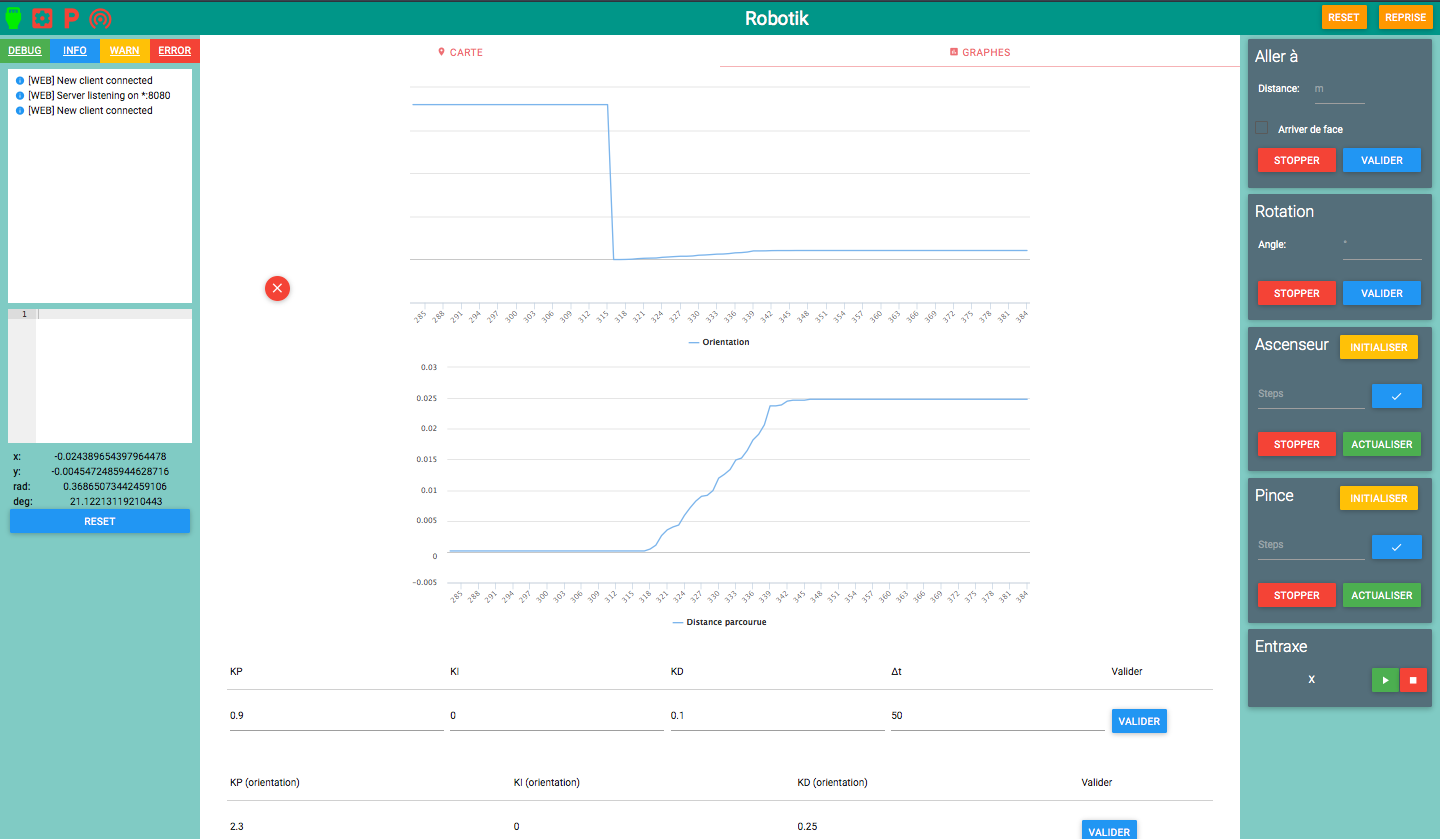
\includegraphics[width=140mm]{assets/debug.png}%
		\caption{Interface de gestion du robot}%
	\end{figure}


	\newpage

	\section{Ce qu'il faut améliorer}
	Sur ce module, nous sommes pour le moment assez satisfaits de la puissance de calcul disponible et nous resterons donc sur le même type de support physique avec le même système d'exploitation pour l'année prochaine. Cependant il y a quelques points que l'on souhaite changer :

	\begin{itemize}
		\item \textbf{Une Raspberry Pi 2 au lieu d'une Odroid C1 :} Les différences entre ces deux cartes ne sont pas significatives, cependant, le support et la communauté sont bien plus importants sur la Raspberry Pi 2, ce qui lui assure une pérennité dans le projet : Si une personne reprend le club sans qu'il y ait de suivi, elle pourra plus facilement reprendre la même carte car elle est plus utilisée et qu'une simple recherche sur internet donne beaucoup d'informations. Ainsi le travail fait sur cette machine a plus de chances d'être réutilisé.
		\item \textbf{ECMAScript 6 vs ECMAScript 5 :} Cette année nous utilisions une norme non-supportée de notre langage de programmation afin de pouvoir utiliser certains avantages disponibles uniquement dans la prochaine version. Cependant cela ajoutait beaucoup de complexité et nécessite de configurer son système afin que le code soit transpilé juste pour devoir tester le code. L'année prochaine nous souhaitons baisser cette complexité. Et donc peut-être faire de l'ES5. Cependant, peut être que NodeJS (le logiciel qui exécute notre code) disposera de nouvelles mises à jour qui lui permettront d'exécuter un script javascript ES6.
		\item \textbf{Interface de gestion et simulateur :} Notre interface de gestion, bien qu'indispensable, pourrait être plus pratique, il est difficile de lui rajouter des fonctionnalités et elle n'est pas adaptée à toutes les tailles d'écrans, en fait elle n'est pas adapté aux tailles d'écrans des développeurs qui devaient dézoomer pour accéder à toutes les fonctionnalités. De plus on manque d'une interface de visualisation en 3D de ce que pense le robot qui pourrait être couplé à un simulateur.
	\end{itemize}
	\ \\
	On est satisfait du travail sur ce module et nous comptons conserver une bonne partie du travail.